\documentclass[12pt,a4paper]{article}
\usepackage[utf8]{inputenc}
\usepackage{amsmath}
\usepackage{amsfonts}
\usepackage{amssymb}
\usepackage{graphicx}
\title{Distributed Whiteboard Report}
\author{Alex Epstein \& Zi Jian Ng}
\begin{document}
\maketitle


\section{Introduction}

The system we present is a collaborative whiteboard where multiple users can simultaneously draw to a single consistent canvas. The network is structured as a single main server with multiple clients: the server maintains a canonical state of the whiteboard and performs user management functions.

From our testing we have established that the whiteboard performs properly under the required conditions. Multiple users are able to access and modify the whiteboard concurrently, and each user sees exactly the same drawings rendered on the whiteboard. Users are able to draw with the main shape tools (line, rectangle, circle, triangle), free line, and enter text. All drawings including text are colourable. 

As additional features, we have implemented a user chat protocol, the ability to load and save a canvas to a file, and the ability for the admin user to kick a particular client by username. Similarly to the canvas itself, the user view of the chat and users list is apparently consistent across clients. 

At an architectural level, we determined during planning that the main non-functional requirements for the system are consistency and responsiveness, while enabling strict control over group membership and the authentication of particular operations. Our approach fulfils these requirements at a small scale. However, the scalability of the current system for a large number of users can be improved, which is discussed in section 4.

\section{System Architecture \& Communication \\Protocols}

The whiteboard protocol was implemented using Java RMI as a callback-oriented architecture. There are two main modules: client and server. 

The client module is responsible for displaying the GUI (\textit{ClientGUI}) and the rendered canvas (\textit{InteractiveCanvas}), and hosts a remote object (\textit{InteractiveCanvasManager}) responsible for communication with the server, both issuing and receiving method invocations. 

The server is a single class (\textit{RemoteWhiteboard}) which handles the canonical state of the whiteboard and user management functions. The canonical whiteboard state is represented as a list of \textit{Drawing} objects, each of which contain the necessary information to render them (origin, size, colour, etc.), along with a client signature and a timestamp. 

An example drawing, involving a call from client to server, is shown in figure \ref{fig:draw}.

\begin{figure}[h]
\frame{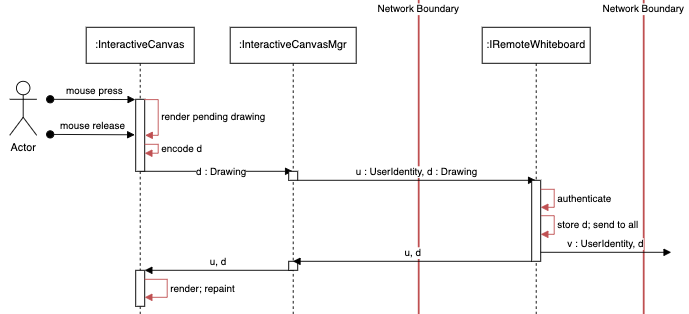
\includegraphics[width=\textwidth]{senddrawingdiagram.png}}
\caption{Example interaction diagram of an authenticated user submitting a drawing}
\label{fig:draw}
\centering
\end{figure}

In figure \ref{fig:draw}, a drawing of a rectangle is recognised by a mouse listener acting on the client's canvas. When the mouse is released, this triggers the canvas to send the drawing to its manager, which invokes the remote method in the server. In the server call, the canvas manager sends its \textit{UserIdentity} along with the \textit{Drawing}. The server subsequently verifies the user's identity, which consists of a username and password, then adds the drawing to its internal representation of the canvas. Then, the server issues a callback invocation to each of the client processes containing the drawing, which notifies them to render the new drawing.

At the client side, new drawings are received by the canvas manager, which adds them to a queue and notifies the canvas that drawings are pending. On receiving this notification, each drawing is drawn permanently to a flat image, which the client's canvas actually renders (the ``canvas flat"). 

\begin{figure}[h]
\frame{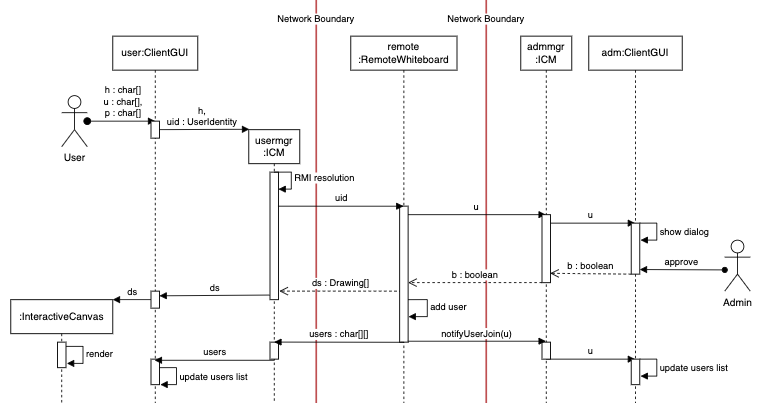
\includegraphics[width=\textwidth]{userjoindiagram.png}}
\caption{Example interaction diagram of a new user successfully joining the server}
\label{fig:join}
\centering
\end{figure}

For user management operations, the procedure is similar, as shown in figure \ref{fig:join}. Once a user has initiated a join request and been approved by the administrator, the server invokes callback methods in each client to notify them of a new user: similarly for when a user leaves, or a user sends a message in chat; the client uses one-way unicast and the server uses one-way multicast to update the global state. 


\section{Implementation Details}

For the purposes of authentication, we have implemented a simple protocol which consists of the passing of \textit{UserIdentity} objects between client and server. Each identity object contains the username and password of the sending client, and the server stores duplicates of these items in addition to the admin's credentials to verify certain operations. Obviously, this is not secure, but the whiteboard is neither persistent nor a high-integrity system, and so plain-text was considered adequate. Users are also somewhat protected against spoofing by the fact that duplicate usernames are disallowed.

The \textit{Drawing} package was designed to ensure small message sizes, and therefore throughput, and therefore the scalability of the system. Each drawing is represented by the minimum amount of information necessary to render it: in the case of simple shapes, a pair of integer coordinates is sufficient representation. In the case of free lines, a novel compression algorithm was written to minimise the amount of space required, reducing it by 80\% in some cases while preserving all but the most granular details of the line. 

Persistent storage of the canvas is accomplished locally on the client's machine, as a serialised array of drawings presented as a ``.canvas" file. When saving, the client requests the drawings array from the server, and when opening, the (admin) client deserialises the saved file and sends this to the server, which replaces the state with the saved state, changing the view for all clients. The performance bottleneck for this process is the number of \textit{FreeLine} objects in the array, as the size of the other drawings is trivial. However, this has been somewhat mitigated, as shown above.

The admin user is allowed to kick another user by invoking the relevant remote method in the whiteboard server. This removes the user from the server's list of approved users, and notifies the other clients that the user has been disconnected.

We now evaluate the non-functional requirements of the system, considering consistency, scalability, and performance.

\textit{Since requests to the server are served in the order they are received}, there is little possibility that a user will see an inconsistent state unless the notification from the server to the user is lost or interrupted, which is considered a rare event: in this case, the user can disconnect and reconnect to remedy their local state. If a draw request from client to server fails, the drawing client will observe that the figure is not rendered on their local canvas, and so can retry. The order that each draw request arrives to the server is considered canonical, as we cannot rely on clock synchronisation between the clients. In short, barring rare events, the single-server architecture of the system maintains consistency. 

Scalability of the system, though not a major concern, is difficult to assess given that Java RMI's implicit use of multithreading is not specified or standardised. Since all clients use strict unicast communication to and from the server, the server itself is the bottleneck: for each drawing sent by one of the $n$ clients, the server must echo that drawing to all $n$ users, which degrades performance linearly with large $n$ - if each user sends $m$ drawings per second, the server must make $mn^2$ remote method calls per second, in addition to the increased overhead from user management. 

However, this performance hit is mitigated by the fact that \textit{Drawing} objects are sent and stored at the server instead of raw images, greatly reducing message size. The server is \textit{not responsible} for rendering each drawing as an image, which is a substantial consideration: the rendering process runs on the client machine, which experiences less load in general. Although this results in duplicated effort, minimising the server's required throughput is the critical factor, and so this results in greater health of the total system as it scales. 

Other scaling factors are considered in the next section.

\section{Improvements for Future Work}

The whiteboard system is currently only designed for a small number of users to use collaboratively. However, scaling of the system is certainly possible with a few improvements to the protocol, which are discussed in this section. Functional improvements are not discussed because there are simply too many to cover in the present report.

Firstly, the overhead for storage and communication at the server, which is the bottleneck of the system, could be improved with a few strategies. Firstly, once a certain number of drawings are sent to the canvas (roughly 100, for example), the canvas may flatten them to an image to reduce the storage size, as hosting a large number of shapes which are totally occluded represents wasted storage capacity. Essentially, this restricts the size of any canvas to a constant, which means the performance of the system scales only with $n$ rather than the number of existing drawings as well. In addition, we can consider alternative compression algorithms for \textit{FreeLine} drawings, such as a two-dimensional fast Fourier transform. 

A new method for multicast communication other than sequential RMI callbacks might be implemented to reduce the load on the server for new drawings, which is currently linear in the number of users in the system. For example, IP multicast can be exploited to send duplicated messages to each user. This would mean the performance of the server no longer scales with $n$ quadratically, and instead only as a function of total system request frequency $nm$. However, this would require another layer of indirection and the implementation of reliability guarantees, which are not provided by standard IP multicast. 

In general, while RMI is a straightforward and high-level abstraction, in order to make stronger guarantees about reliability and ordering, the communications protocols should be rewritten at a lower level using TCP sockets. This enables the programmer to have explicit control over the control flow of the server, and therefore can enforce stricter ordering on messages, ensuring consistency across the system at the cost of a larger and less maintainable codebase.

Lastly, the security of the system could be vastly improved: instead of sending passwords as cleartext, they should ideally be transmitted and stored as salted hashes or using some other similar cryptographic method. Similarly, we could implement a message numbering system to reduce the feasibility of replay attacks. Additionally, to prevent the possibility of denial-of-service attacks, the administrator should have the option to randomly assign a remote reference to the server rather than the default value of ``//localhost/Whiteboard". However, we considered that such security measures were currently outside the scope of this project.

\end{document}










